\chapter{Propuesta}\label{chapter:proposal}
    Para la solución de los problemas planteados se propone definir un \emph{pipeline} que contará con 6 etapas principales.
    que abarcan desde la carga de los documentos, el procesado de los mismos para ser almacenados en una base de datos. Realizar un agrupamiento para la detección de las principales temáticas presentes en el corpus y particularmente los documentos más representativos para cada una de ellas. Posteriormente estos documentos son compendiados a modo de un resumen extractivo y, a su vez, se obtienen las referencias bibliográficas correspondientes. En la ultima fase se realiza un post procesado mediante un LLM para generar un resumen abstractivo a partir del texto que se obtuvo en la fase anterior. Finalmente se junta dicho resumen con las referencias bibliograficas obtenidas. En figura () se muestra un diagrama del \emph{pipeline} descrito

    \begin{figure}[H]    
        \centering
        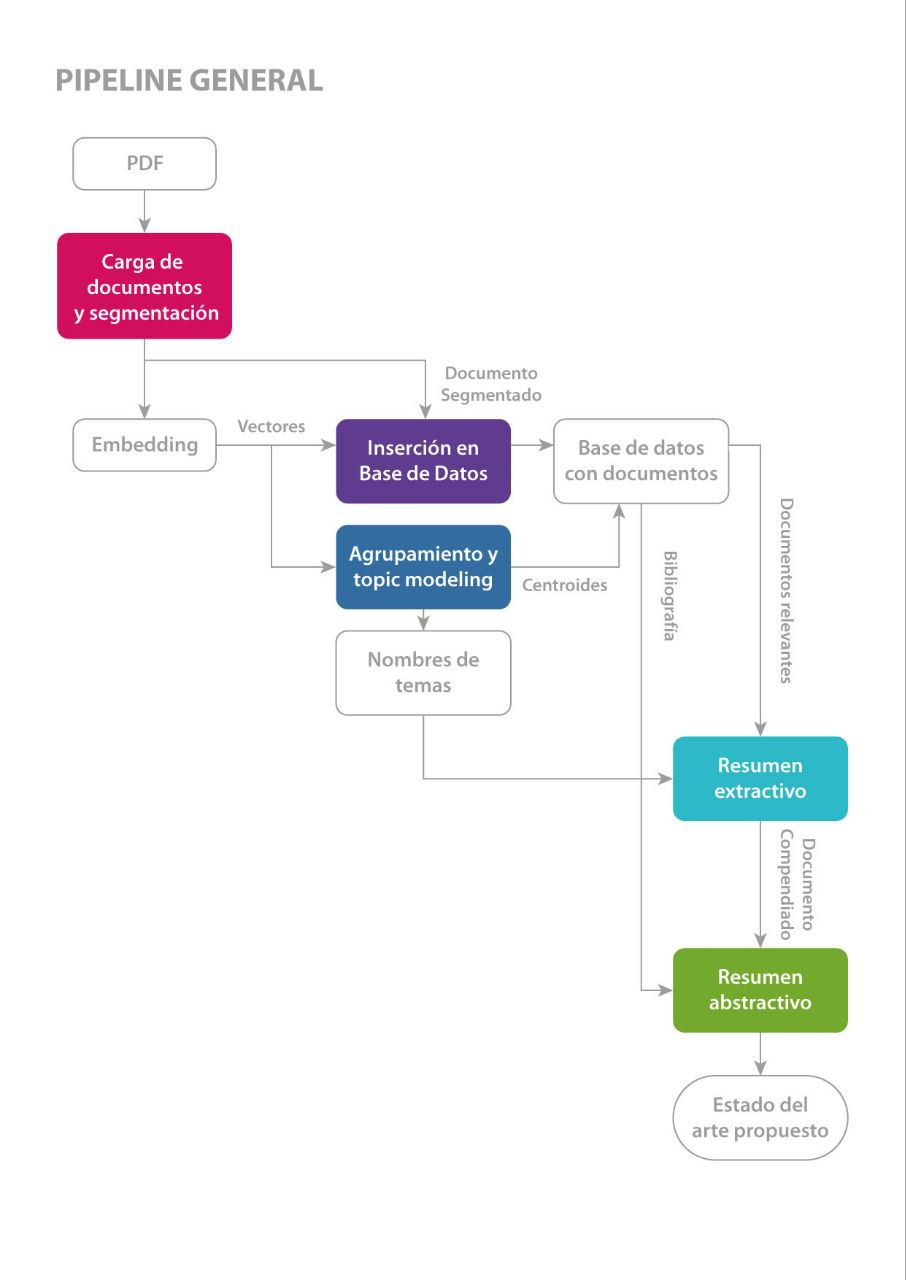
\includegraphics[scale = 1]{Figures/pipeline_general.png}
        \caption*{}
    \end{figure}
    

    \section{Primera fase: Carga de documentos} 
    La primera fase del \emph{pipeline} se centra en la carga los documentos. Se realiza además una segmentación de la información (en oraciones, párrafos u otro método de segmentación del texto) con el objetivo de representarla de manera granular. Con el fin de que sea más fácil agrupar semánticamente la información representada en los documentos. Esto será primordial para una fase posterior que se enfoca en la recuperación de la información.

    \begin{figure}[H]    
        \centering
        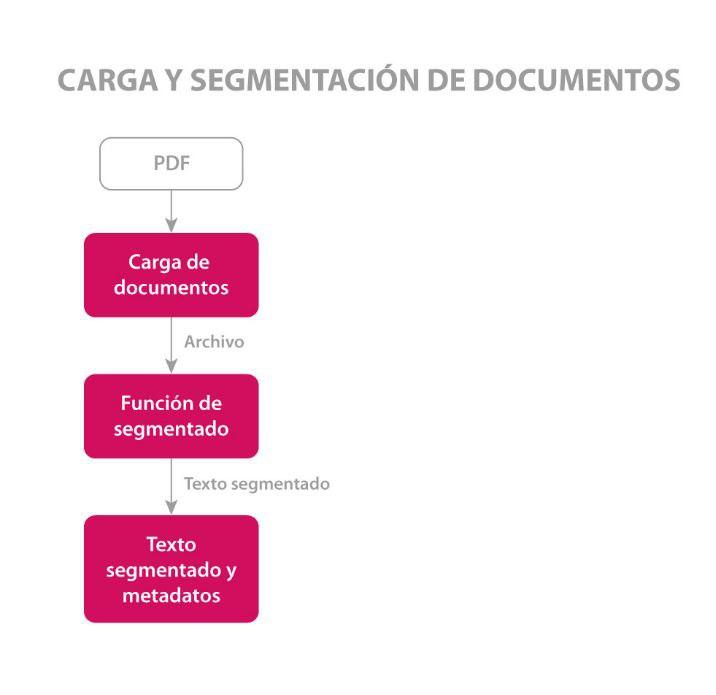
\includegraphics[scale = 1]{Figures/pipeline_1.png}
        \caption*{}
    \end{figure}
    
    \section{Segunda Fase: \emph{Embeddings}}
    Esta segunda fase comprende la conversión de la información previamente preprocesada en \emph{Embeddings de texto}.
    La representación del texto de esta manera permite obtener una abstracción de las ideas contenidas en los documentos. 
    Para ello se decidie utilizar el modelo `all-MiniML-L6-v2' que, de acuerdo con las pruebas de \emph{MTEB} [\cite{leaderboard}] obtiene buenos resultados sin altos requerimientos de tiempo y recursos computacionales. Estos \emph{embeddings} son unos vectores de dimensión 384 que serán almacenados en una base de datos vectorial para facilitar el acceso a estos y la realización de búsquedas por similaridad. \emph{Embedings} que traten del mismo tema se han de encontrar mas cerca entre si que \emph{embeddings} que representen conceptos diferentes.

    \begin{figure}[H]    
        \centering
        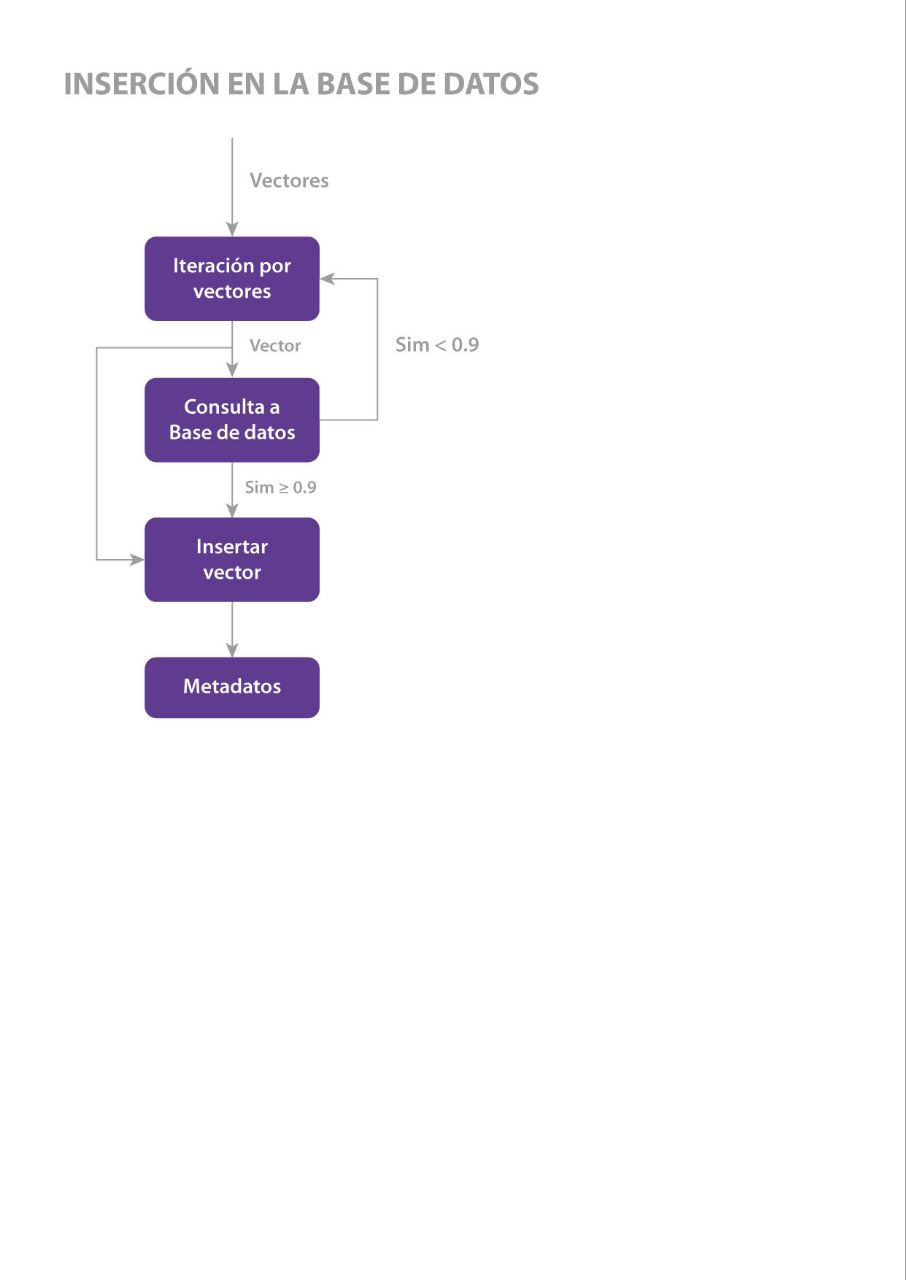
\includegraphics[scale = 1]{Figures/pipeline_2.png}
        \caption*{}
    \end{figure}

    \section{Tercera Fase: Inserción en la Base de datos}
    Los vectores que representan los documentos se almacenan en una base de datos vectorial que permite de manera eficiente acceder tanto a los documentos como a los metadatos de los mismos. A la vez que facilita el uso de búsqueda de similaridad utilizando otros vectores. Durante la inserción de los vectores se hace uso de esta funcionaliada para evitar introducir información redundante en la base de datos. De esta manera son descartados los vectores que no aportan información nueva a la base de conocimiento.

    \begin{figure}[H]    
        \centering
        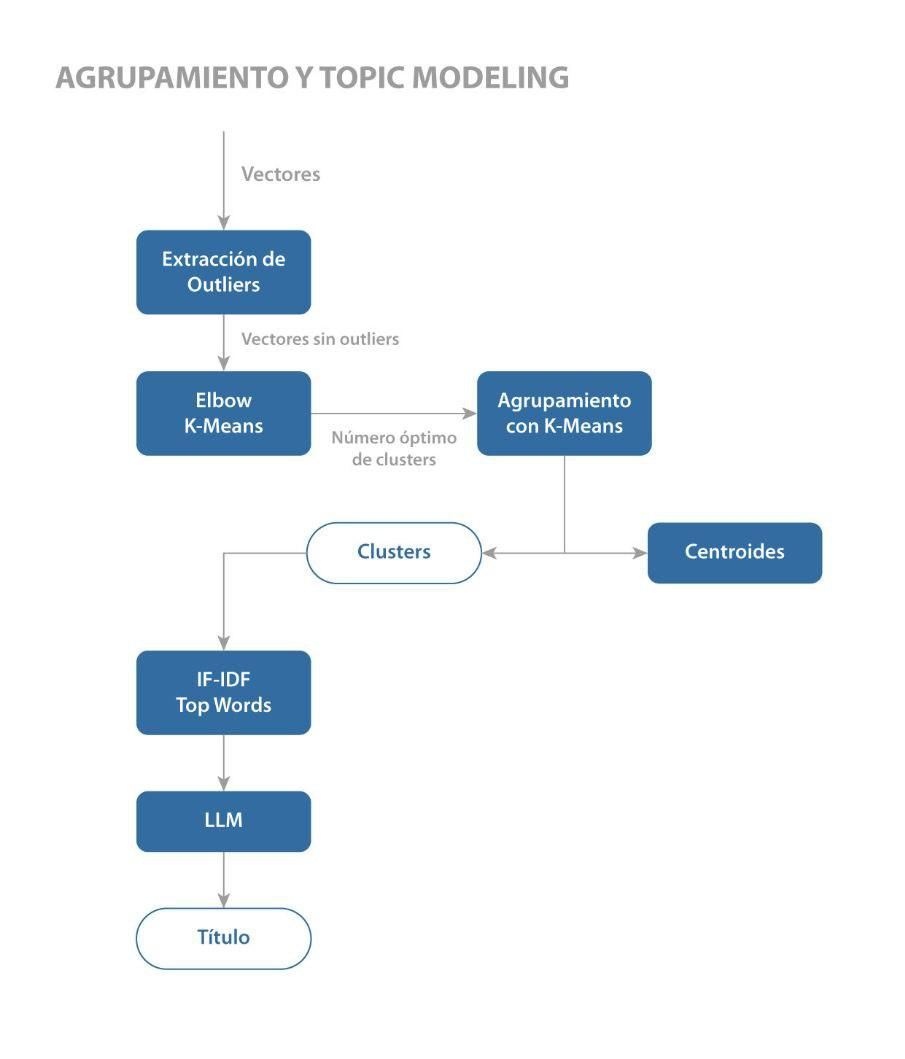
\includegraphics[scale = 1]{Figures/pipeline_3.png}
        \caption*{}
    \end{figure}

    \section{Cuarta Fase: Agrupamiento por temas}
    Una vez obtenidos los \emph{embeddings} es necesario agrupar la información en una serie de temas, para ello se procesan mediante un algoritmo de \emph{clustering} que se encarga de agruparlos atendiendo a la similaridad. Se hace uso del método del codo, una técnica utilizada en la clasificación de datos para determinar el número óptimo de clústeres\footnote{Un centroide es el punto representativo de un grupo de datos, calculado como el promedio de las características de todos los puntos pertenecientes a ese grupo, y se utiliza como el centro o punto focal para asignar datos a un clúster específico en algoritmos de agrupamiento.}. Este método se basa en calcular la distorsión promedio de cada clúster, que es la distancia de cada elemento con su centroide correspondiente. Al graficar la distorsión en función del número de clústeres, se busca identificar el punto donde la curva forma un "codo", indicando que agregar más clústeres no aportaría una mejora significativa. Una vez se obtiene la cantidad óptima de clústeres, se procede a generar un agrupamiento con todos los documentos y, por ende, los centroides que representan cada tema. Estos centroides están representados a su vez como vectores de la misma dimensionalidad que los \emph{embeddings} generados, por tanto; pueden ser utilizados para realizar una búsqueda en la base de datos vectorial que contiene los documentos. De esta manera se pueden recuperar los documentos que, conceptualmente estén más relacionados con el tema que los engloba. En esta fase además, una ves que se obtienen los distintos clústeres, se puedeutilizar una tabla \emph{TF-IDF} para obtener las palabras más relevantes para un tema. Con estas palabras, haciendo uso de un LLM se genera una propuesta de título para el tema.

    \begin{figure}[H]    
        \centering
        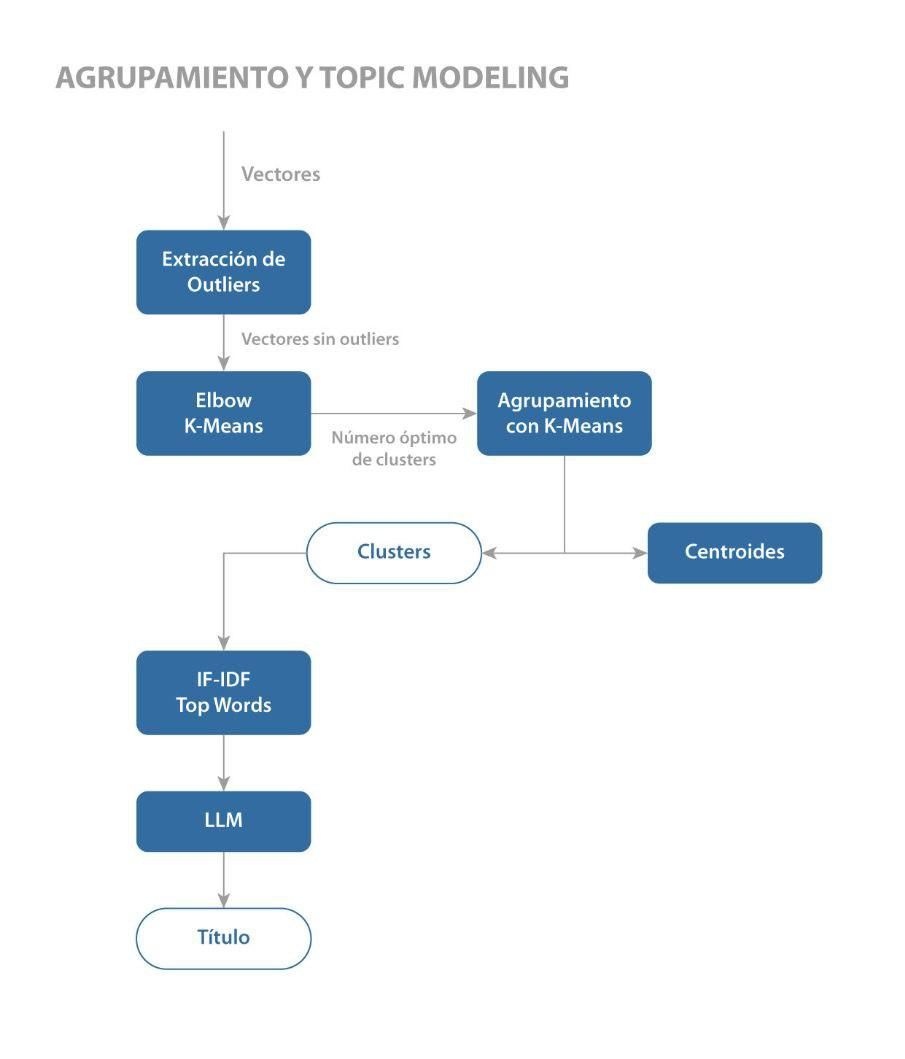
\includegraphics[scale = 1]{Figures/pipeline_3.png}
        \caption*{}
    \end{figure}

    \section{Quinta Fase: Resumen extractivo} 
    Los documentos más relevantes para un tema son recuperados tras realizar una búsqueda en la base de datos utilizando como referencia los centroides asociados a cada clúster. Estos documentos son agrupados a modo de resumen extractivo de cada uno de los temas detectados en el paso anterior (nótese que en este cointexto, un documento no necesariamente tiene que ser la totalidad del documento original, pues fueron segmentados en la primera fase). El proceso de extracción devuelve también los metadatos del elemento recuperado. Dichos metadatos actúan a modo de referencia al documento original que contiene la información de cada elemento recuperado por el sistema de bases de datos. De esta manera se garantiza una bibliografía consistente con la información recuperada. Estas referencias no serán procesadas por las futuras fases del \emph{pipeline}.
    
    \begin{figure}[H]    
        \centering
        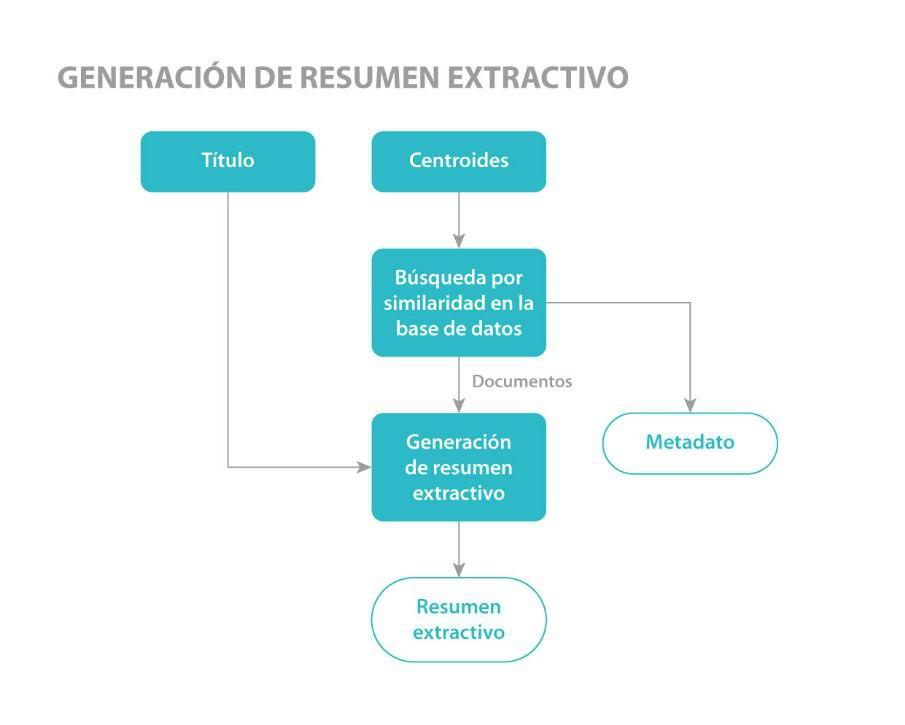
\includegraphics[scale = 1]{Figures/pipeline_4.png}
        \caption*{}
    \end{figure}

    \section{Sexta Fase: Resumen extractivo}
    El resumen extractivo generado en la fase anterior se utiliza como parte del \emph{prompt} que es utilizado por el LLM para generar el texto del resumen absrtactivo asociado a un tema.

    Los textos obtenidos son organizados acorde a un formato de salida predefinido: una enumeración de los temas definidos (con el título sugerido para el tema en la fase de agrupamiento por temas) y posteriormente el resumen correspondiente a cada tema. Se añaden también las referencias a los documentos utilizados obtenidos de la base de datos.

    \begin{figure}[H]    
        \centering
        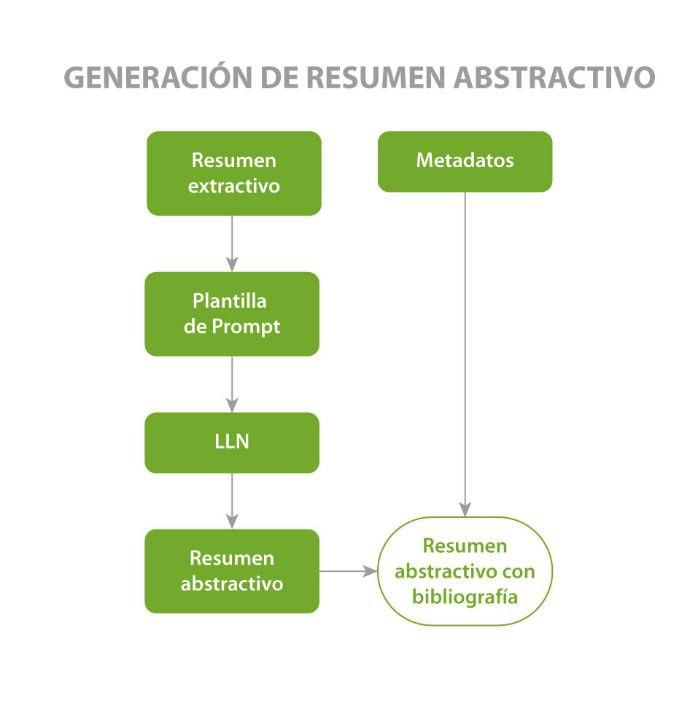
\includegraphics[scale = 1]{Figures/pipeline_5.png}
        \caption*{}
    \end{figure}
